To aid the computationally minded reader, we give below some charts of the trigraded homotopy groups of $\mathrm{kq}_2$.
These charts are meant to be read in concert with those of \cite[\S 6.5]{Kong}, and the notation here matches that in Kong's work.
Indeed, all of the information within these charts is easily accessed within Kong's work, and we merely repackage it here.

We focus on the homotopy groups $\pi_{p,q,w} (\mathrm{kq}_2 \otimes C\ta)$ and $\pi_{p,q,w}(\mathrm{kq}_2)$ for $p=0$ and $p=-1$.
In the language of \cite{Kong}, this corresponds to a focus on \emph{coweights} $0$ and $-1$.

\begin{figure}[ht]
\centering
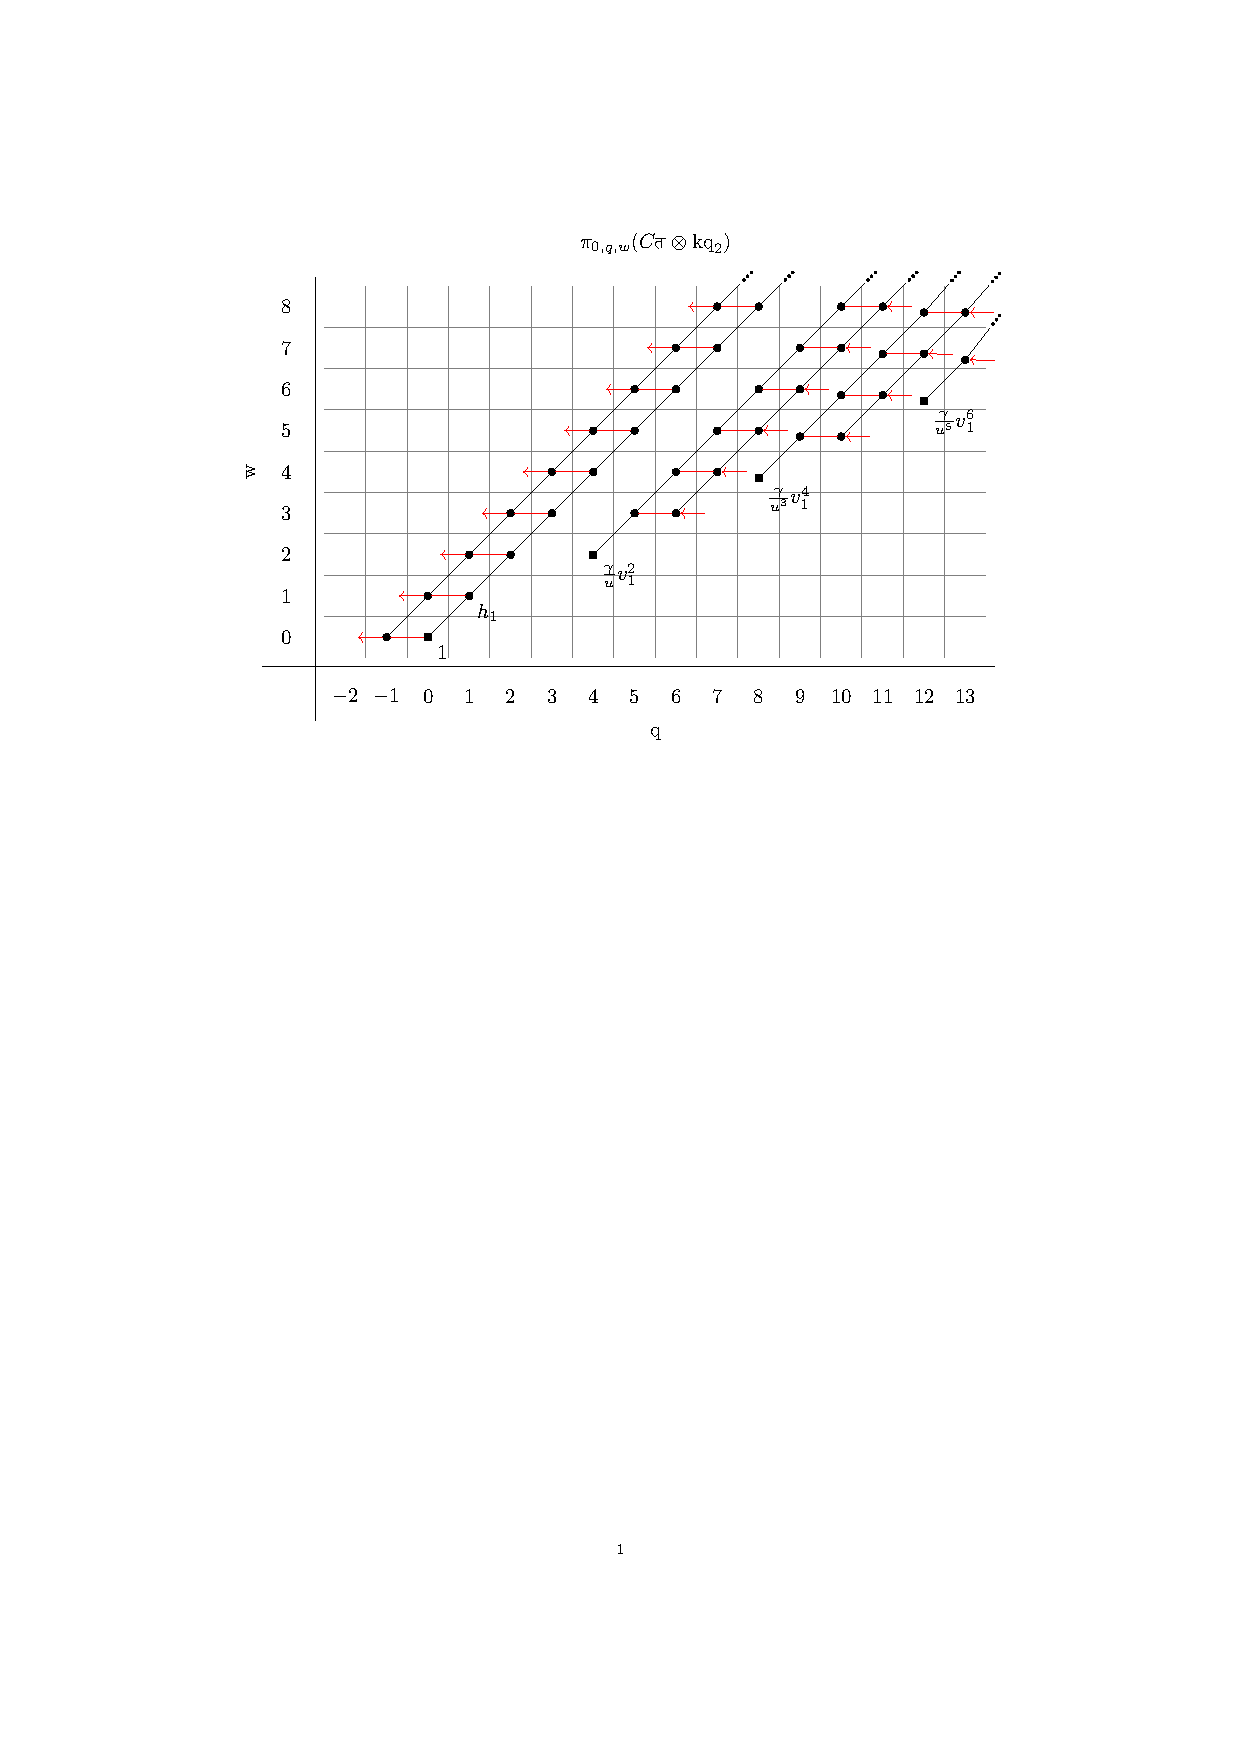
\includegraphics[trim=100 470 100 100, clip, width=\textwidth, scale=0.6]{kqChart1.pdf}
\end{figure}


Red lines denote multiplication by $a \in \pi_{0,-1,0} \Ss$.  Black lines denote multiplication by the motivic $\eta:\mathbb{G}_m \to \Ss$, which in our grading convention lives in $\pi_{0,1,1} \Ss$.

\newpage

\begin{figure}[ht]
\centering
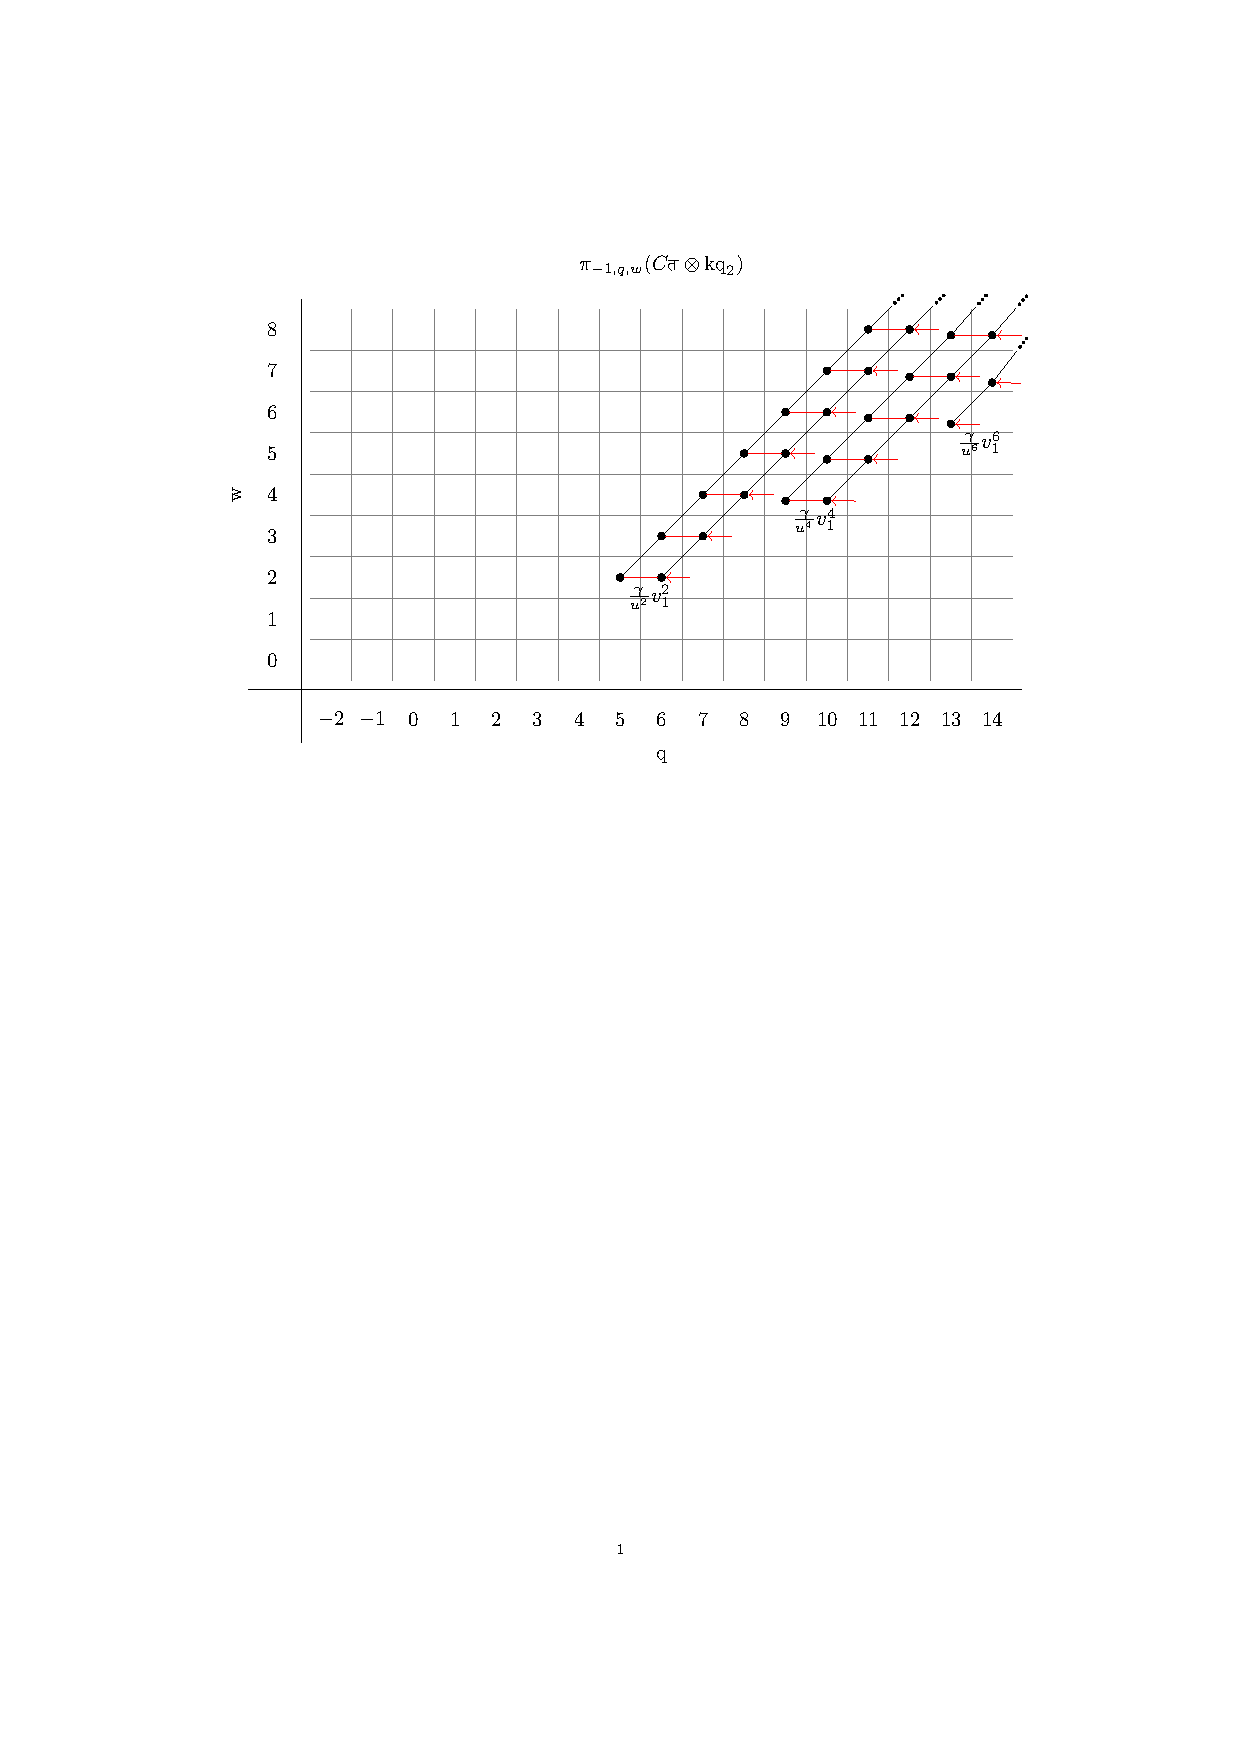
\includegraphics[trim=100 470 100 120, clip, width=\textwidth, scale=0.6]{kqChart2.pdf}
\end{figure}

Below, we depict some of the $\mathrm{E}_{\infty}$-page of the $\ta$-Bockstein spectral sequence for $\pi_{*,*,*} \mathrm{kq}_2$.
We follow the convention introduced in \cite[\S A.2]{Boundaries} and \cite{BurklundExtension} of using blue symbols to denote $\ta$-torsion classes, while black symbols denote $\ta$-torsion free classes.
In particular, black symbols contribute not only to the homotopy group corresponding to the box in which they appear, but also to the groups corresponding to boxes directly below where they appear.
In the language of \cite{Kong}, the blue dots in our charts contain information about which dots on the $\mathrm{E}_1$-page of the $C_2$-effective spectral sequence are targets of differentials, as opposed to sources of differentials.

\begin{figure}[ht]
\centering
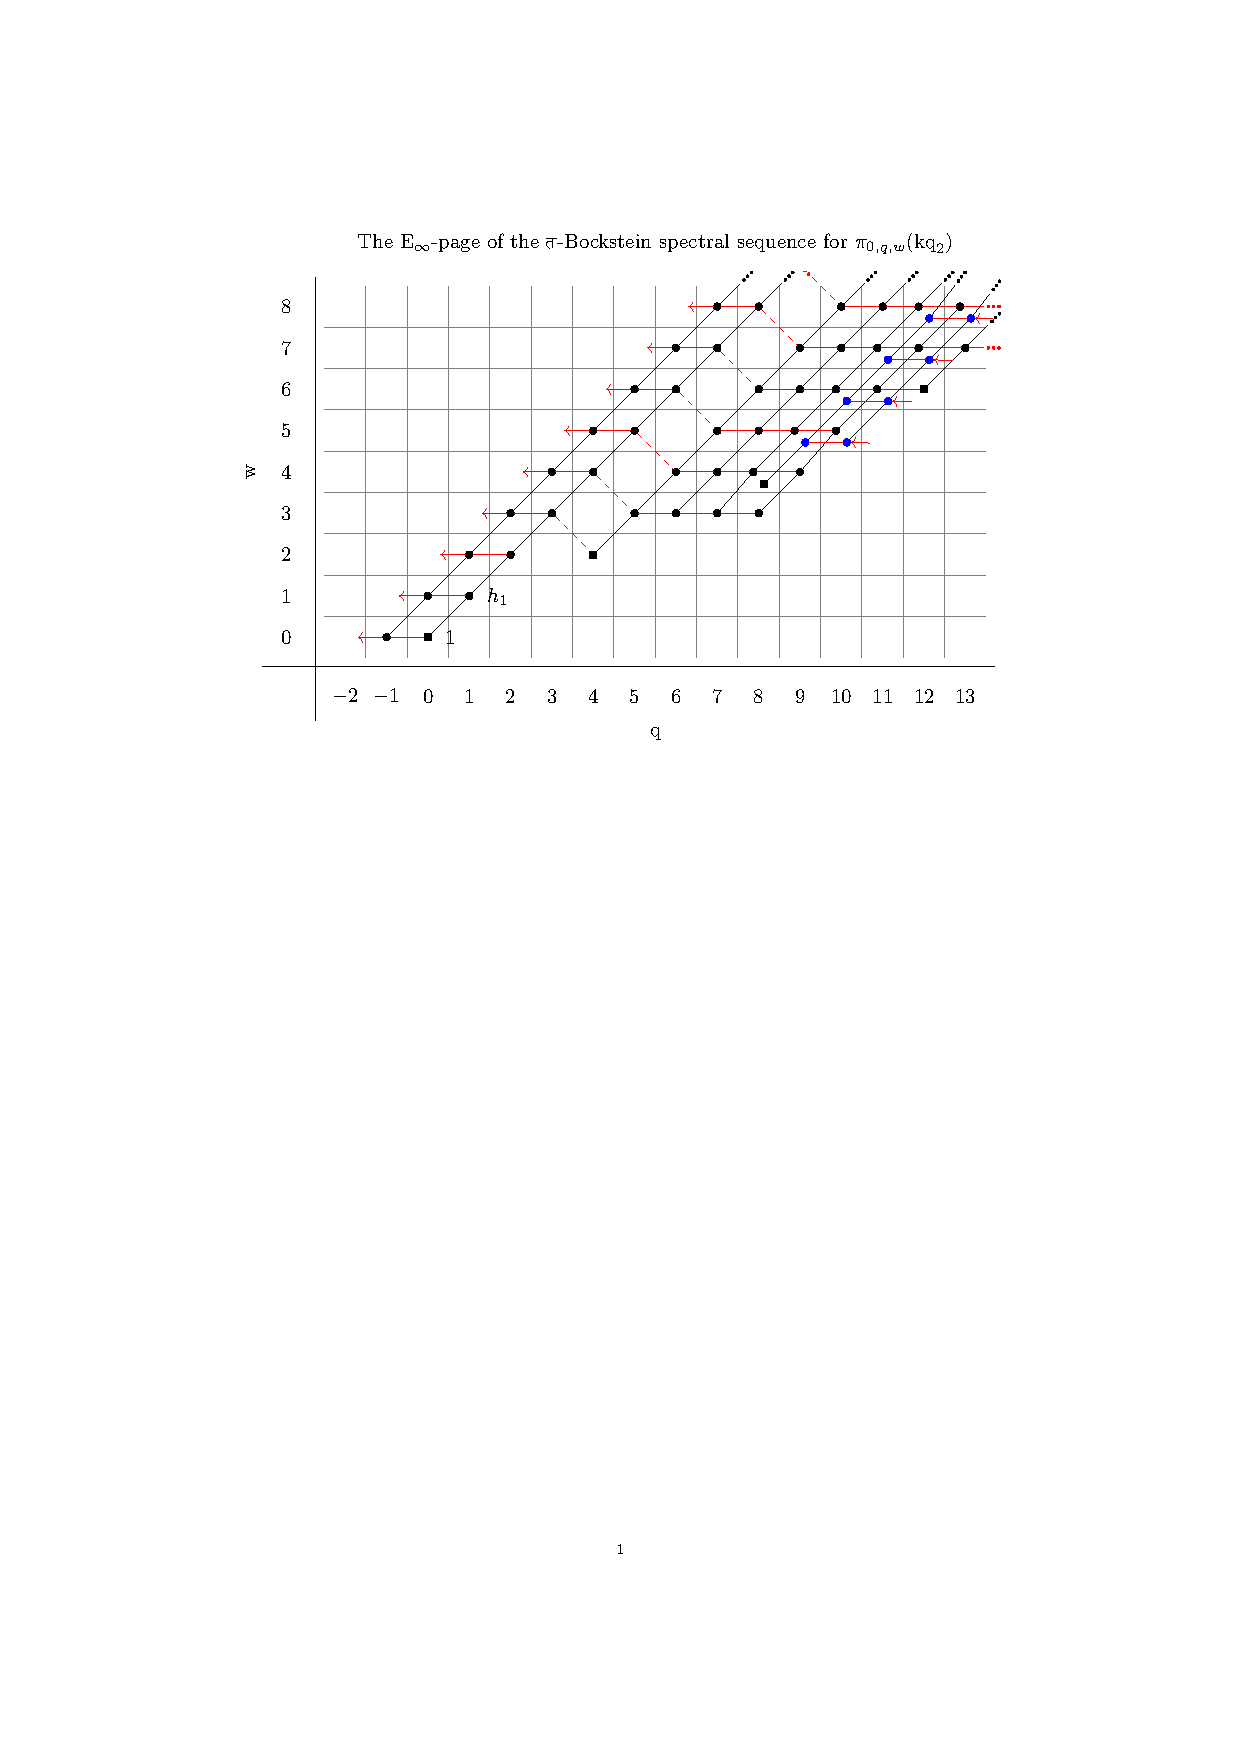
\includegraphics[trim=100 470 100 100, clip, width=\textwidth, scale=0.6]{kqChart3.pdf}
\end{figure}

\begin{figure}[ht]
\centering
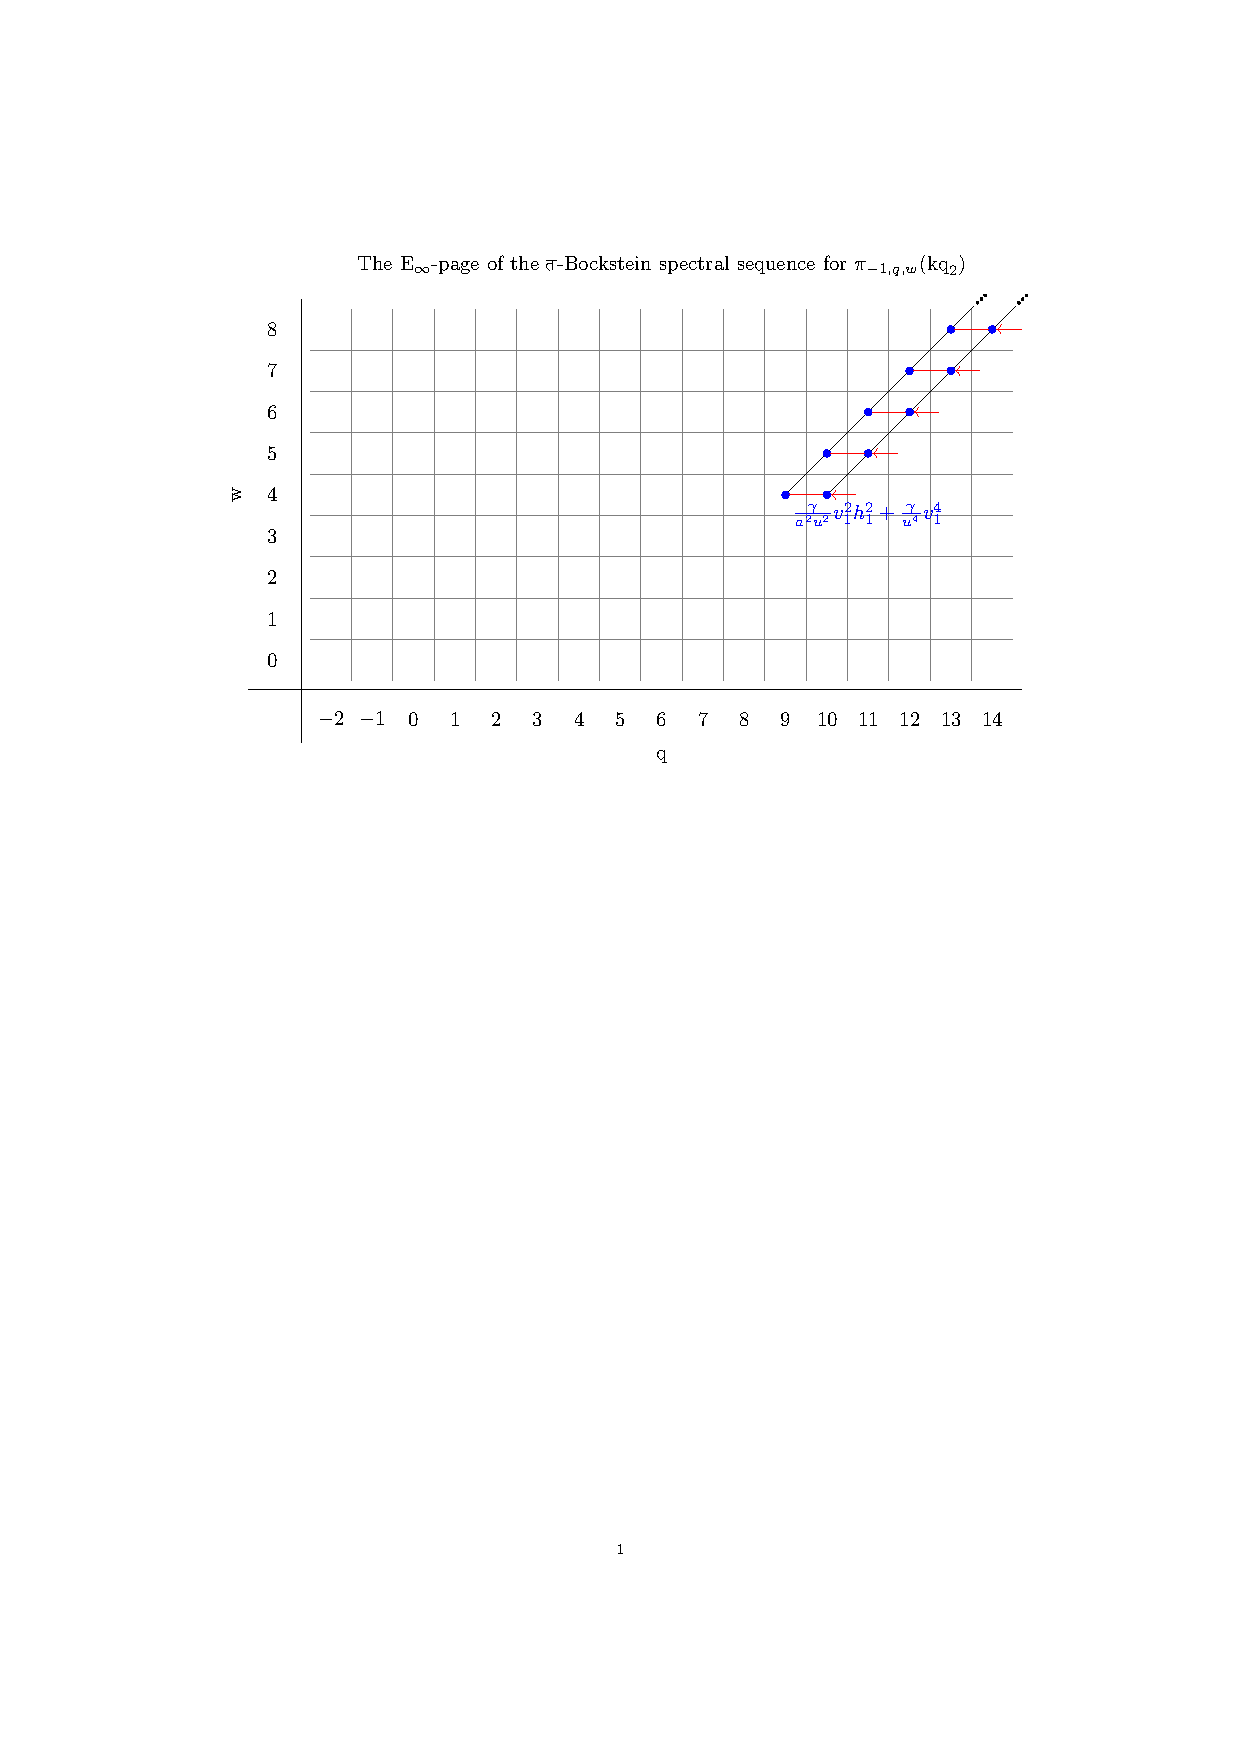
\includegraphics[trim=100 470 100 100, clip, width=\textwidth, scale=0.6]{kqChart4.pdf}
\end{figure}

\begin{rmk}
The groups $\pi_{-1,*,*}\mathrm{kq}_2$ and $\pi_{0,*,*}\mathrm{kq}_2$ assemble, via the multiplication by $a$ long exact sequence, into the homotopy groups $\pi_{0,*,*}\left(Ca \otimes \mathrm{kq}_2\right)$.  These groups in turn record the bigraded homotopy of the $\C$-motivic $\mathrm{kq}_2$.  The reader may note an interesting extension, of the form 
\[2 \mathbb{Z}_2[\tau] \oplus \tau \mathbb{Z}_2[\tau] \to \mathbb{Z}_2[\tau] \to \mathbb{F}_2,\]
which appears when computing $\pi_{0,8,*}(\mathrm{kq}_2^{\wedge} \otimes Ca)$.
This extension is related to the orange dashed line in the final chart of \cite{Kong}.
\end{rmk}




\begin{comment}
In this section, we note that the $\ta$-Bockstein spectral sequence for $\pi_{***} kq^{\wedge}_2$ is an incarnation of the \emph{effective} spectral sequence for $(ko_{C_2})^{\wedge}_2$ studied in CITE.
The trigraded homotopy groups $\pi_{***} kq$ record both the differentials and extension problems present in this spectral sequence.
To give a visual representation of the structure of these homotopy groups, we record the hyperplane $\pi_{4,*,*} kq$ in FIGURE.
This may be directly compared to figure BLAH of CITE, where the integer $4$ is referred to as the `coweight.'

We next indicate how, upon inverting the class $a \in \pi_{0,-1,0} (kq)^{\wedge}_2$, the resulting bigraded homotopy groups record the classical $\Ft$-Adams spectral sequence for $(\Phi^{C_2} ko_{C_2})^{\wedge}_2 \simeq \oplus_{k \ge 0} \Sigma^{4k} \Zt$.
Extension problems in this Adams spectral sequence are invisible to the classical bigraded homotopy groups $\pi_{p,q,q} (kq)^{\wedge}_2$, but are recorded in trigraded homotopy via BLAH.

\begin{rmk}
For a general Galois cellular $X$, we do not expect (?) such a close relationship between the effective spectral sequence and $\ta$-Bockstein spectral sequence.  For example, the $\ta$-Bockstein spectral sequence for the sphere spectrum is more closely related to the Chow--Novikov spectral sequence of CITE.  \todo{justify this... refer to something about Chow--Novikov or something in the sphere or both?}
\end{rmk}

\begin{prop}
There is an additive isomorphism
$\pi_{*,*,*}(kq^{\wedge}_2 \otimes C\ta) \cong \uZt[v_1^2] \oplus \uFt[h_1,v_1^2]{h_1}$,
where $|v_1|=(2,2,2)$ and $|h_1|=(0,1,1)$.
\end{prop}

\begin{proof}
Consider the $2$-completed slice tower converging to $kq^{\wedge}_2$, which as described in CITE has associated graded a direct sum of Eilenberg--MacLane spectra indexed by products of $h_1$ and $v_1^2$.
Since $C\ta$ is a finite complex, we may tensor this tower with $C\ta$ to obtain a tower converging to $kq^{\wedge}_2 \otimes C\ta$.
By CITE, the $E_1$-page of the spectral sequence associated to this tower is $\uZt[v_1^2] \oplus \uFt[h_1,v_1^2]{h_1}$.
No possible differentials or additive extension problems can occur, for tridegree reasons.
\end{proof}

\begin{prop}
The $\ta$-Bockstein spectral sequence
$$\pi_{p,q,w}(kq^{\wedge}_2 \otimes C\ta)[\ta] \implies \pi_{p,q,w}(kq^{\wedge}_2)$$
degenerates at the $\sE_2=\sE_{\infty}$-page.  The $d_1$ differential is determined under the Leibniz rule by the relations
\begin{enumerate}
\item $d_1(u^2)=\ta a^2  u h_1$
\item $d_1(v_1^2)=\ta u h_1^3$
\end{enumerate}
Upon inverting $\ta$, this spectral sequence is identified with the effective spectral sequence for $\pi_{p+q\sigma}((ko_{C_2})^{\wedge}_2)$.
\end{prop}

\begin{proof}
The $d_1$ differential lands in $\ta$-torsion free groups, so its value can be determined after inverting $\ta$.
One then reads off the two claimed $d_1$ differentials from CITE, remembering as always that $\tau=\ta u$ and $\rho = \ta a$. \todo{maybe nicer to directly use the below remark}
To see that these two $d_1$ differentials determine all other $d_1$-differentials via the Liebniz rule, see Remark CITE.

The first page $\ta^{-1} E_1$ of the $\ta$-inverted Bockstein spectral sequence agrees with the first page of the effective spectral sequence studied in CITE, and $\ta^{-1} d_1$ agrees with the $d_1$ differential in the effective spectral sequence CITE.  Kong proves CITE that the effective spectral sequences converges and collapses at $\sE_2=\sE_{\infty}$.  Since the $\ta$-inverted spectral sequence also converges, it must converge to the same groups.  Any additional non-zero differentials in the $\ta$-inverted spectral sequence would make this impossible, and so the $\ta$-inverted spectral sequence must also collapse at $\sE_2$.  Any potential differential in the $\ta$-Bockstein spectral sequence has target a $\ta$-torsion free group, and so would be detected after inverting $\ta$.
\end{proof}

\begin{rmk}
The $d_1$ differentials above can be seen as arising from two independent sources.  The first differential $d_1(u^2) = \ta a^2 u h_1$ arises from a slice differential in $kgl$, and is detected under the natural map $kq \to kgl$.
The second differential $d_1(v_1^2)=\ta u h_1^3$ is detected under the map $kq \to kq \otimes Ca$, and so is essentially $\C$-motivic in origin.
Under the correspondence between cellular $\C$-motivic homotopy and even $MU$-synthetic spectra CITE, one may read this $d_1$-differential off from the $d_3$-differential $d_3(v_1^2)=h_1^3$ in the classical Adams--Novikov spectral sequence for for $\pi_*(ko)$.
\end{rmk}

\begin{cor}
There are differentials
$$d_1(\frac{\theta}{a^i u^j}) = \begin{cases} \frac{\theta}{a^{i-2} u^{j+1}} \ta \text{ if } j=4k+2 \\ 0 \text{ otherwise}. \end{cases}$$
\end{cor}

\begin{proof}
\end{proof}

There are many hidden extensions in the $\ta$-Bockstein spectral sequence.  After inverting $\ta$, these extensions are determined in CITE.  In order to analyze $a^{-1} (kq)_2^{\wedge}$, we will need the following hidden extension:

\begin{prop}
There is a relation
$ a^2 \eta \ta= 2a \ta \in \pi_{***} (kq)^{\wedge}_2$,
which corresponds to a hidden extension
$a^2 h_1 \ta = 2a$
in the $\sE_{\infty}$-page of the $\ta$-Bockstein spectral sequence.
\end{prop}

\begin{proof}
\end{proof}

The following result relates the homotopy groups of $a^{-1} (kq)^{\wedge}_2$ with the classical $\mathbb{F}_2$-Adams spectral sequence for $(\Phi^{C_2} ko_{C_2})^{\wedge}_2 \simeq \oplus_{k \ge 0} \Sigma^{4k} \Zt$.  We use Pstragowski's language of $\Ft$ synthetic spectra to encode this Adams spectral sequence.

\begin{thm}
There is an isomorphism of bigraded rings
$$\pi_{*,0,*} a^{-1} (kq)^{\wedge}_2 \cong \pi_{*,*} \nu_{\Ft}((\Phi^{C_2} ko_{C_2})_2^{\wedge}).$$ \todo{work out how the degrees shear}
Explicitly, this ring is the $\ta$-adic completion of $\mathbb{Z}_2[x,y,\ta]/(\ta x = 2),$
where $|x|=(0,1)$, $|\ta|=(0,-1)$, and $|y|=(4,0)$.
Under the map $(kq)^{\wedge}_2 \to a^{-1} (kq)^{\wedge}_2$, $x$ and $y$ are the images of $a h_1 \in \pi_{0,0,1} (kq)^{\wedge}_2$ and $u^2 v_1^2 \in \pi_{4,0,} (kq)^{\wedge}_2$, respectively.
\end{thm}

\begin{rmk}
There is no $\ta$-torsion in the bigraded homotopy of $a^{-1} (kq)^{\wedge}_2$.  Equivalently, all of the $\ta$-torsion present in the homotopy of $(kq)^{\wedge}_2$ is killed by some power of $a$.  This is a reflection of the fact that the Adams spectral sequence for $(\Phi^{C_2} ko_{C_2})_2^{\wedge}$ degenerates at the $\sE_2$-page, with no higher differentials.
\end{rmk}


CHARTS PUT BELOW WITHOUT CHANGE


We indicate the trigraded homotopy groups $\pi_{p,q,w} (C\ta \otimes kq_2^{\wedge})$ for $p=0$ and $p=-1$.  These may be compared with CITE, where they correspond to the $E_1$-page of the effective spectral sequence in coweights $0$ and $-1$.

\begin{center}
\begin{sseqpage}[ xscale=0.7, yscale=0.7, x range = {-2}{13}, y range = {0}{8}, x tick step = 1, y tick step = 1, class labels = {right}, classes = fill, grid = crossword, x label = {q}, y label = {w}, title = {$\pi_{0,q,w}(C\ta \otimes kq^{\wedge}_2)$}, class labels = {below right = 0.00 em} ]

\class[rectangle, "1"](0,0) 
\class[](-1,0) \structline[red](0,0)
\draw [->,red] (-1,0) -- (-2+0.3,0);

\class["h_1"](1,1)
\class[](0,1) \structline[red]
\draw [->,red] (0,1) -- (-1+0.3,1);

\foreach \i in {2,...,10} { \class(\i, \i) \class(\i-1,\i) \structline[red]  \draw [->,red] (\i-1,\i) -- (\i-2+0.3,\i);}
\foreach \i in {1,...,10} {\structline(\i,\i)(\i-1,\i-1) \structline(\i-1,\i)(\i-2,\i-1)}

\class[rectangle, "\frac{\gamma}{u} v_1^2"](4,2)
\foreach \i in {1,...,10} {
\class(4+\i,2+\i) \structline(3+\i,1+\i)
\class(5+\i,2+\i) \structline[red](4+\i,2+\i)
\draw[->,red](6-0.3+\i,2+\i)--(5+\i,2+\i);
}
\foreach \i in {2,...,9} {
\structline(5+\i,2+\i)(4+\i,1+\i)
}



\class[rectangle, yshift=-0.1, "\frac{\gamma}{u^3} v_1^4"](8,4)
\foreach \i in {1,...,10} {
\class[yshift=-0.1](8+\i,4+\i) \structline(7+\i,3+\i)
\class[yshift=-0.1](9+\i,4+\i) \structline[red](8+\i,4+\i)
\draw[->,red](10-0.3+\i,4+\i-0.15)--(9+\i,4+\i);
}
\foreach \i in {2,...,9} {
\structline(9+\i,4+\i)(8+\i,3+\i)
}


\class[rectangle, yshift=-0.2, "\frac{\gamma}{u^5} v_1^6"](12,6)
\class[yshift=-0.2](13,7) \structline
\class[yshift=-0.2](14,8) \structline
\draw[->,red](13.7,6.7)--(13,7);


\end{sseqpage}
\end{center}





\begin{center}
\begin{sseqpage}[ xscale=0.7, yscale=0.7, x range = {-2}{14}, y range = {0}{8}, x tick step = 1, y tick step = 1, class labels = {right}, classes = fill, grid = crossword, x label = {q}, y label = {w}, title = {$\pi_{-1,q,w}(C\ta \otimes kq^{\wedge}_2)$}, class labels = {below right = 0.00 em} ]

\class["\frac{\gamma}{u^2} v_1^2"](5,2)
\class(6,2) \structline[red]
\draw[->,red](7-0.3,2)--(6,2);

\foreach \i in {1,...,10} {
\class(5+\i,2+\i) \structline(4+\i,1+\i)
\class(6+\i,2+\i) \structline[red](5+\i,2+\i)
\draw[->,red](7-0.3+\i,2+\i)--(6+\i,2+\i);
}
\foreach \i in {1,...,9} {
\structline(6+\i,2+\i)(5+\i,1+\i)
}

\class[yshift=-0.1, "\frac{\gamma}{u^4} v_1^4"](9,4)
\class[yshift=-0.1](10,4) \structline[red]
\draw[->,red](11-0.3,4-0.15)--(10,4);

\foreach \i in {1,...,10} {
\class[yshift=-0.1](9+\i,4+\i) \structline(8+\i,3+\i)
\class[yshift=-0.1](10+\i,4+\i) \structline[red](9+\i,4+\i)
\draw[->,red](11-0.3+\i,4+\i-0.15)--(10+\i,4+\i);
}
\foreach \i in {1,...,9} {
\structline(10+\i,4+\i)(9+\i,3+\i)
}

\class[yshift=-0.2, "\frac{\gamma}{u^6} v_1^6"](13,6)
\draw[->,red](13.7,5.7)--(13,6);
\class[yshift=-0.2](14,7) \structline
\class[yshift=-0.2](15,8) \structline
\draw[->,red](14.7,6.7)--(14,7);

%\class["\frac{\gamma}{u^6} v_1^6"](13,6)

\end{sseqpage}
\end{center}

In these charts, red lines denote multiplication by $a \in \pi_{0,-1,0} \Ss$.  Black lines denote multiplication by the motivic $\eta:\mathbb{G}_m \to \Ss$, which in our grading convention lives in $\pi_{0,1,1} \Ss$.


%% \newpage

Below are charts, for $p=0,-1$, of the $E_{\infty}$-pages of the $\ta$-Bockstein spectral sequence converging to $\pi_{p,q,w} kq_2^{\wedge}$.  The first of these charts may be compared to CITE.

\begin{center}
\begin{sseqpage}[ xscale=0.7, yscale=0.7, x range = {-2}{14}, y range = {0}{8}, x tick step = 1, y tick step = 1, class labels = {right}, classes = fill, grid = crossword, x label = {q}, y label = {w}, title = {$\pi_{-1,q,w}(kq^{\wedge}_2)$}, class labels = {below right = 0.00 em} ]

\class[blue, "\frac{\gamma}{a^2u^2}v_1^2h_1^2 + \frac{\gamma}{u^4}v_1^4"](9,4)
\class[blue](10,4) \structline[red]
\draw[->,red](11-0.3,4)--(10,4);

\foreach \i in {1,...,10} {
\class[blue](9+\i,4+\i) \structline(8+\i,3+\i)
\class[blue](10+\i,4+\i) \structline[red](9+\i,4+\i)
\draw[->,red](11-0.3+\i,4+\i)--(10+\i,4+\i);
}
\foreach \i in {1,...,9} {
\structline(10+\i,4+\i)(9+\i,3+\i)
}

\end{sseqpage}
\end{center}



\begin{center}
\begin{sseqpage}[ xscale=0.7, yscale=0.7, x range = {-2}{13}, y range = {0}{8}, x tick step = 1, y tick step = 1, class labels = {right}, classes = fill, grid = crossword, x label = {q}, y label = {w}, title = {$\pi_{0,q,w}(kq^{\wedge}_2)$} ]

\class[rectangle, "1"](0,0) 
\class[](-1,0) \structline[red](0,0)
\draw [->,red] (-1,0) -- (-2+0.3,0);

\class["h_1"](1,1)
\class[](0,1) \structline[red]
\draw [->,red] (0,1) -- (-1+0.3,1);

\foreach \i in {2,...,10} { \class(\i, \i) \class(\i-1,\i) \structline[red]  \draw [->,red] (\i-1,\i) -- (\i-2+0.3,\i);}
\foreach \i in {1,...,10} {\structline(\i,\i)(\i-1,\i-1) \structline(\i-1,\i)(\i-2,\i-1)}


\class[rectangle](4,2) \structline[red, dashed](4,2)(3,3)
\class(5,3) \structline[red,dashed](4,4) \structline(4,2)
\class(6,3) \structline[red] \class(7,3) \structline[red] \class(8,3) \structline[red]
\class(6,4) \structline[red,dashed](5,5) \structline(5,3) 
\class(7,4) \structline[red] \structline(6,3) 
\class(8,4) \structline[red] \structline(7,3)
\class(9,4) \structline[red] \structline(8,3)
\class(7,5) \structline[red,dashed](6,6) \structline(6,4)
\class(8,5) \structline[red] \structline(7,4)
\class(9,5) \structline[red] \structline(8,4)
\class(10,5) \structline[red] \structline(9,4)
\class(8,6) \structline[red,dashed](7,7) \structline(7,5)
\class(9,6) \structline[red] \structline(8,5)
\class(10,6) \structline[red] \structline(9,5)
\class(11,6) \structline[red] \structline(10,5)
\class[rectangle](12,6) \structline[red]
\class(9,7) \structline[red,dashed](8,8) \structline(8,6)
\class(10,7) \structline[red] \structline(9,6)
\class(11,7) \structline[red] \structline(10,6)
\class(12,7) \structline[red] \structline(11,6)
\class(13,7) \structline[red] \structline(12,6)
\class(14,7) \structline[red]
\class(10,8) \structline[red,dashed](9,9) \structline(9,7)
\class(11,8) \structline[red] \structline(10,7)
\class(12,8) \structline[red] \structline(11,7)
\class(13,8) \structline[red] \structline(12,7)
\class(14,8) \structline[red] \structline(13,7)
\class(11,9) \structline(10,8)
\class(12,9) \structline(11,8)
\class(13,9) \structline(12,8)
\class(14,9) \structline(13,9)

\class[rectangle, yshift=-0.2](8,4) %\structline[orange, dashed](8,3)
\foreach \i in {1,...,10} {
\class[blue, yshift=-0.2](8+\i,4+\i) \structline(7+\i,3+\i,-1)
\class[blue, yshift=-0.2](9+\i,4+\i) \structline[red](8+\i,4+\i,-1)
\draw[->,red](10-0.3+\i,4+\i-0.3)--(9+\i,4+\i,-1);
}
\foreach \i in {2,...,9} {
\structline(9+\i,4+\i,-1)(8+\i,3+\i,-1)
}


\end{sseqpage}
\end{center}


The homotopy groups of $kq_2^{\wedge} \otimes Ca$ record the $\C$-motivic homotopy of $kq_2^{\wedge}$, or in other words the classical Adams--Novikov spectral sequence for $ko^{\wedge}_2$.  Note the extension
$$2 \mathbb{Z}[\tau] \oplus \tau \mathbb{Z}[\tau] \to \mathbb{Z}[\tau] \to \mathbb{F}_2[\tau]/\tau^{2},$$
which appears when computing $\pi_{0,8,*}(kq_2^{\wedge} \otimes Ca)$.
\end{comment}